\documentclass[tikz,border=8pt]{standalone}
\usepackage{xcolor}
\usetikzlibrary{calc,arrows.meta,backgrounds}
\definecolor{bg}{HTML}{1B1F27}
\definecolor{fg}{HTML}{E6EDF3}
\definecolor{dim}{HTML}{9AA5B1}
\definecolor{c1}{HTML}{7BC47F}
\definecolor{c2}{HTML}{E5826F}
\definecolor{cb}{HTML}{6EA8FE}
\definecolor{cd}{HTML}{B39DDB}
\definecolor{feat}{HTML}{F0C060}
\begin{document}
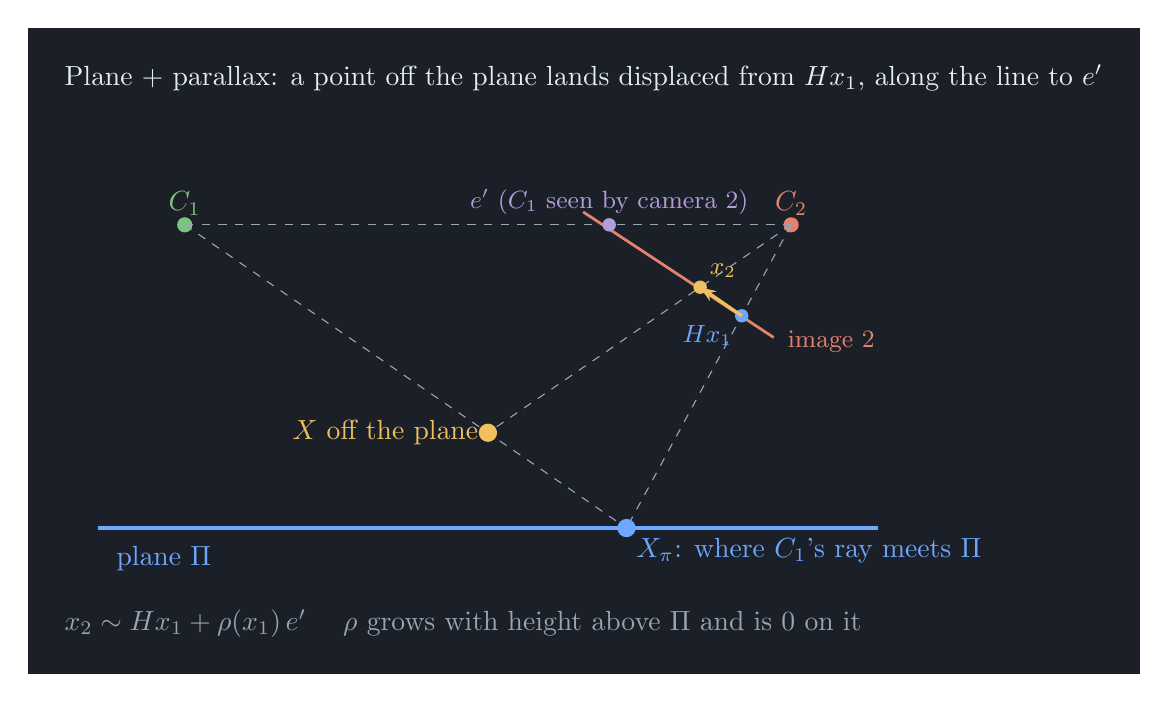
\begin{tikzpicture}[show background rectangle, background rectangle/.style={fill=bg}, inner frame sep=10pt, every node/.style={text=fg}, scale=1.1]
% side view: the plane is a line
\coordinate (C1) at (1.5,5);
\coordinate (C2) at (8.5,5);
\coordinate (X) at (5,2.6);
\coordinate (P) at (6.6,1.5);
\draw[cb, line width=1.4pt] (0.5,1.5) -- (9.5,1.5);
\node[text=cb, anchor=west] at (0.6,1.15) {plane $\Pi$};
\fill[c1] (C1) circle (2.5pt); \node[text=c1, above] at (C1) {$C_1$};
\fill[c2] (C2) circle (2.5pt); \node[text=c2, above] at (C2) {$C_2$};
\draw[dim, dashed] (C1) -- (X) -- (P);
\draw[dim, dashed] (C2) -- (X);
\draw[dim, dashed] (C2) -- (P);
\draw[dim, dashed] (C2) -- (C1);
\fill[feat] (X) circle (3pt); \node[text=feat, left] at (X) {$X$ off the plane};
\fill[cb] (P) circle (3pt); \node[text=cb, below right] at (P) {$X_\pi$: where $C_1$'s ray meets $\Pi$};

% image 2: the points on the image line
\draw[c2, line width=1pt] (6.1,5.15) -- (8.3,3.7);
\node[text=c2, font=\small, anchor=west] at (8.35,3.65) {image 2};
\coordinate (e) at (6.4,5);
\coordinate (hx) at (7.93,3.95);
\coordinate (x2) at (7.45,4.28);
\fill[cd] (e) circle (2.2pt); \node[text=cd, font=\small, above] at (e) {$e'$ ($C_1$ seen by camera 2)};
\fill[cb] (hx) circle (2.2pt); \node[text=cb, font=\small, below left] at (hx) {$Hx_1$};
\fill[feat] (x2) circle (2.2pt); \node[text=feat, font=\small, above right] at (x2) {$x_2$};
\draw[-{Stealth[length=2mm]}, line width=1.2pt, feat] (hx) -- (x2);
\node[anchor=west] at (0,6.7) {Plane + parallax: a point off the plane lands displaced from $Hx_1$, along the line to $e'$};
\node[anchor=west, text=dim] at (0,0.4) {$x_2\sim Hx_1+\rho(x_1)\,e'$ \quad $\rho$ grows with height above $\Pi$ and is $0$ on it};
\end{tikzpicture}
\end{document}
